\documentclass[11pt]{article}

\usepackage[dvipdfmx]{graphicx}
\usepackage{fancyhdr}
\usepackage{here}
\usepackage{comment}
\usepackage{mathtools}
\usepackage{amsmath, amssymb}
\usepackage{type1cm}
\usepackage{multirow}
\usepackage{enumerate}
% 上下に2.5cm、左右に20cmの余白を取る
\usepackage[top=30mm, bottom=30mm, left=20mm, right=20mm]{geometry}
\usepackage{listings} %,jlisting日本語のコメントアウトをする場合jlisting(もしくはjvlisting)が必要
%ここからソースコードの表示に関する設定
\lstset{
  basicstyle={\ttfamily},
  identifierstyle={\small},
  commentstyle={\smallitshape},
  keywordstyle={\small\bfseries},
  ndkeywordstyle={\small},
  stringstyle={\small\ttfamily},
  frame={tb},
  breaklines=true,
  columns=[l]{fullflexible},
  numbers=left,
  xrightmargin=0zw,
  xleftmargin=3zw,
  numberstyle={\scriptsize},
  stepnumber=1,
  numbersep=1zw,
  lineskip=-0.5ex
}


\newif\iffigure
%\figurefaulse
\figuretrue
%select show the figure or not

\makeatletter
\def\@cite#1{\textsuperscript{#1)}}
\def\@biblabel#1{#1)}
\makeatother

\newcommand{\DATE}[3]{#1年#2月#3日} %month, day, year
\newcommand{\TheDay}{\DATE{2020}{11}{17}}
\newcommand{\Header}{中須賀・船瀬研究室 輪講資料}

\title{卒業研究進捗報告} %最終発表
\date{\TheDay}
\author{
B4 西本 慎吾%\thanks{shingo_n@space.t.u-tokyo.ac.jp}
}

%ヘッダの指定:
\pagestyle{fancy}

\begin{document}
\maketitle
\thispagestyle{fancy}
\lhead[\Header]{\Header} % ヘッダ左側
%\chead[偶数ページの引数]{奇数ページの引数} %ヘッダ中央
\rhead[\TheDay]{\TheDay} %ヘッダ右側
%\lfoot[偶数ページの引数]{奇数ページの引数} %フッタ左側
%\cfoot[偶数ページの引数]{奇数ページの引数} %フッタ中央
%\rfoot[偶数ページの引数]{奇数ページの引数} %フッタ右側


%abstは修正
\begin{abstract}
   To improve the reliability of nano-satellites, it is essential 
   to fix satellite failures which are generated in design phase and
   manufacturing phase.
   Nevertheless, fault analysis depends on human ability or experiences, 
   and the process of identifying failures causes requires considerable 
   human resources and time.
   This research proposes a new approach to support identifying failure causes
   of satellite based on the model of signal, electricity and physical interaction
   between subsystem or components in satellites. The effectiveness of the approach
   is proved by applying it to a simple satellite model and showing the process
   to identify failure cause based on the approach. \\

   %要修正
  超小型衛星の信頼性向上のためには,地上試験によって
  設計や製造過程での不良を事前に発見し,不具合の改修,対策を十分に
  行うことが重要である.
  一方で,不具合分析が個人の知識や経験に大きく依存するため,
  経験が浅いエンジニアや衛星に関する知識の乏しいエンジニアが
  故障原因の特定を十分に行うことは困難である.
  
  本研究では,電気・信号・物理量の流れで表現した
  コンポーネント間の接続関係のモデル化,テレメトリ及びコマンド
  がコンポーネント間を伝達する経路のモデル化を行う.
  また,これらのモデルを用いて故障原因を特定する
  方法(確認すべきテレメトリ,打つべきコマンド)の提示を行い,
  簡易的な衛星モデルを用いて有効性を検証する.

\end{abstract}

\section{はじめに}  
 %発表時にどのような意見が欲しいのか補足する
現在,コマンドとテレメトリをベースにして行う衛星の不具合分析を
支援する手法を検討している.\\
以下の章では,
コンポーネント間の情報の流れを信号や電気,物理現象の流れで表現した
接続関係のモデル化,
コマンドとテレメトリの衛星内部での情報伝搬の流れのモデル化,
そのモデルを用いた不具合分析について説明し,今後の方針を示す.

\section{研究背景} 
\subsection{超小型衛星の信頼性の低さ}

超小型衛星の開発が大学や小企業の中で盛んになってきている.
これまでは教育目的が主であったが,商用利用や革新的なミッションへの応用も
増えてきている\cite{Langer2016}.
一方で現状の超小型衛星は中・大型衛星と比較して軌道上での不具合の確率は高く,
2002から2016の間に打ち上がった
270のCubesatのうち,139のミッションが失敗している\cite{Langer2016}.\\
これらの不具合は,大学衛星が宇宙環境での使用を保証されていない
民生部品を使用することも多いため,軌道上での部品の故障によって
発生すると考えられてきた.しかし,
実際には多くが設計や製造過程に起因する
不具合であることが知られている\cite{Venturini2017}.
軌道上での不具合の根本原因に対する調査(Figure \ref{fig:cause of failure})では,
民生部品の品質の不確定性が原因であったものはわずか17%であり,
それ以外の多くが設計や,地上試験の不足に起因するものである\cite{Venturini2017}.

%ここにできれば具体的な衛星の故障の例を持ってくれると良い
\begin{figure}[H]
   \centering
      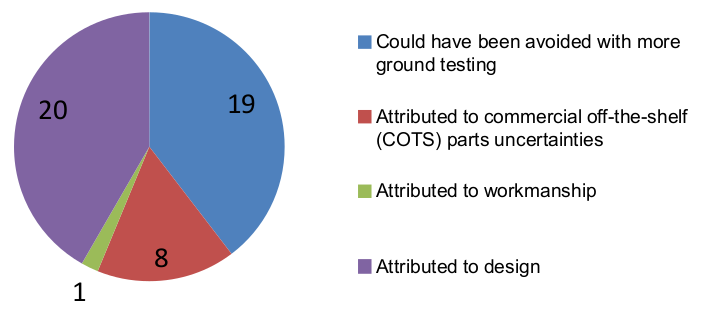
\includegraphics[height=4.5cm]{figure/cause_of_failure.png}
      \caption{故障原因に関するインタビュー結果\cite{Venturini2017}}
      \label{fig:cause of failure}
\end{figure}

%ここへのつながり
また,大学衛星が商用利用や革新的なミッションに
挑戦するためには,超小型衛星のメリットである
コストの低さを十分に確保しながら,
ほどよい信頼性を実現することが,重要であると考えられている\cite{SHIRASAKA2011}.\\
故障に設計や製造の不良が含まれていることを考えると,
超小型衛星の「ほどよい信頼性」の評価を行うためには,
従来用いられてきた
各コンポーネントごとの信頼度の組み合わせでは不十分である.
そこで,設計・製造・運用における
信頼度を加味した評価手法が提案されている\cite{SHIRASAKA2011}.
式(\ref{eq:Reliability})が示すように,この評価手法では
製造時の信頼性も重要な要素であると捉えられている.

\begin{equation}
   R_{sat} = R_{des} \times R_{fab} \times R_{comp} \times R_{op} \label{eq:Reliability}
\end{equation}
\begin{table}[H]
   \centering
      \begin{tabular}{cl} 
        $R_{sat}$ & 衛星の真の信頼度\\
        $R_{des}$ & 設計における信頼度\\
        $R_{fab}$ & 製造における信頼度\\
        $R_{comp}$ & 衛星の信頼度(従来の信頼度)\\
        $R_{op}$ & 運用における信頼度
      \end{tabular}
\end{table}

%もうちょいちゃんと考える
\subsection{地上試験における問題}
以上で示したように,不具合の多くが設計,製造などに起因している
という問題がある.
一方で,これは超小型衛星開発のみに限られたことではなく,
中・大型衛星においても大きな問題となっている.
軌道上故障データを分析した結果\cite{SAITO2011}(Figure \ref{fig:error tyoe})
によると,軌道上で
偶発的に発生した故障はわずか11%であり,それ以外は設計,製造などの開発
活動に起因するものであることがわかっている.\\
また,軌道上で発生した不具合が地上試験で
発現しなかった,または発見できなかった原因が以下の
Figure \ref{fig:error cause}のように知られている.
試験設備の不足によるものや,故障発見までの
時間が長く試験で発見することが現実的で無いものに関しては,
コストとリソースの面から試験による対策では限界がある.
一方で,試験モードの不備や,発現していたのにもかかわらず
発見できなかった不具合に関しては
試験に対する習熟度が不足していること,
不具合・リスクの分析が不十分であることが推測される\cite{SAITO2011}.

\begin{figure}[H]
   \centering
      \begin{tabular}{c}
         \begin{minipage}{0.50\hsize}
         \centering
         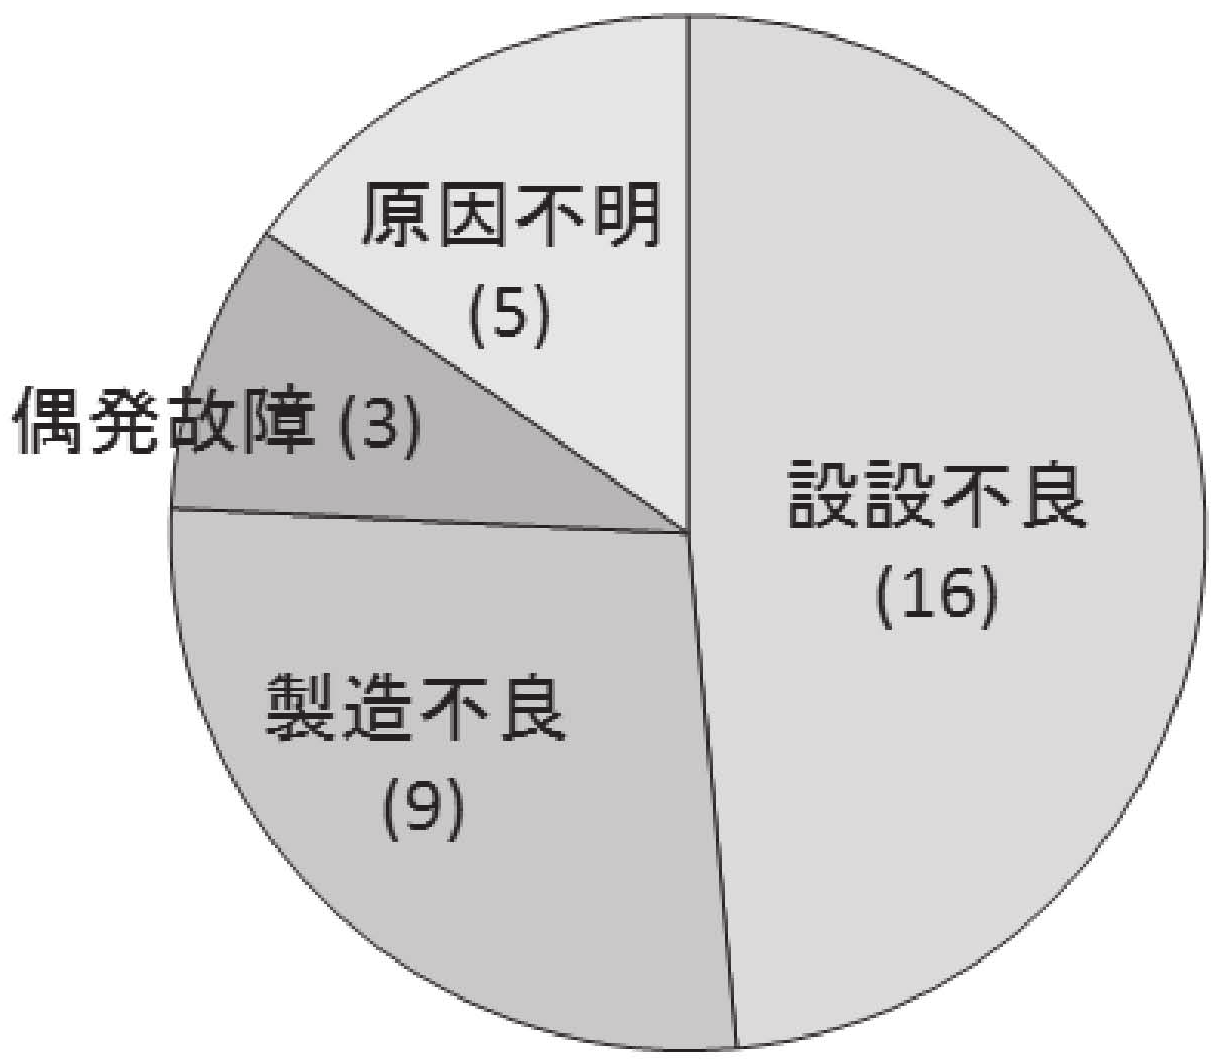
\includegraphics[width=5.5cm]{figure/on_orbit_error_tyoe.png}
            \caption{軌道上故障の原因類型の分布\cite{SAITO2011}}
            \label{fig:error tyoe}
         \end{minipage}
         \begin{minipage}{0.50\hsize}
         \centering
         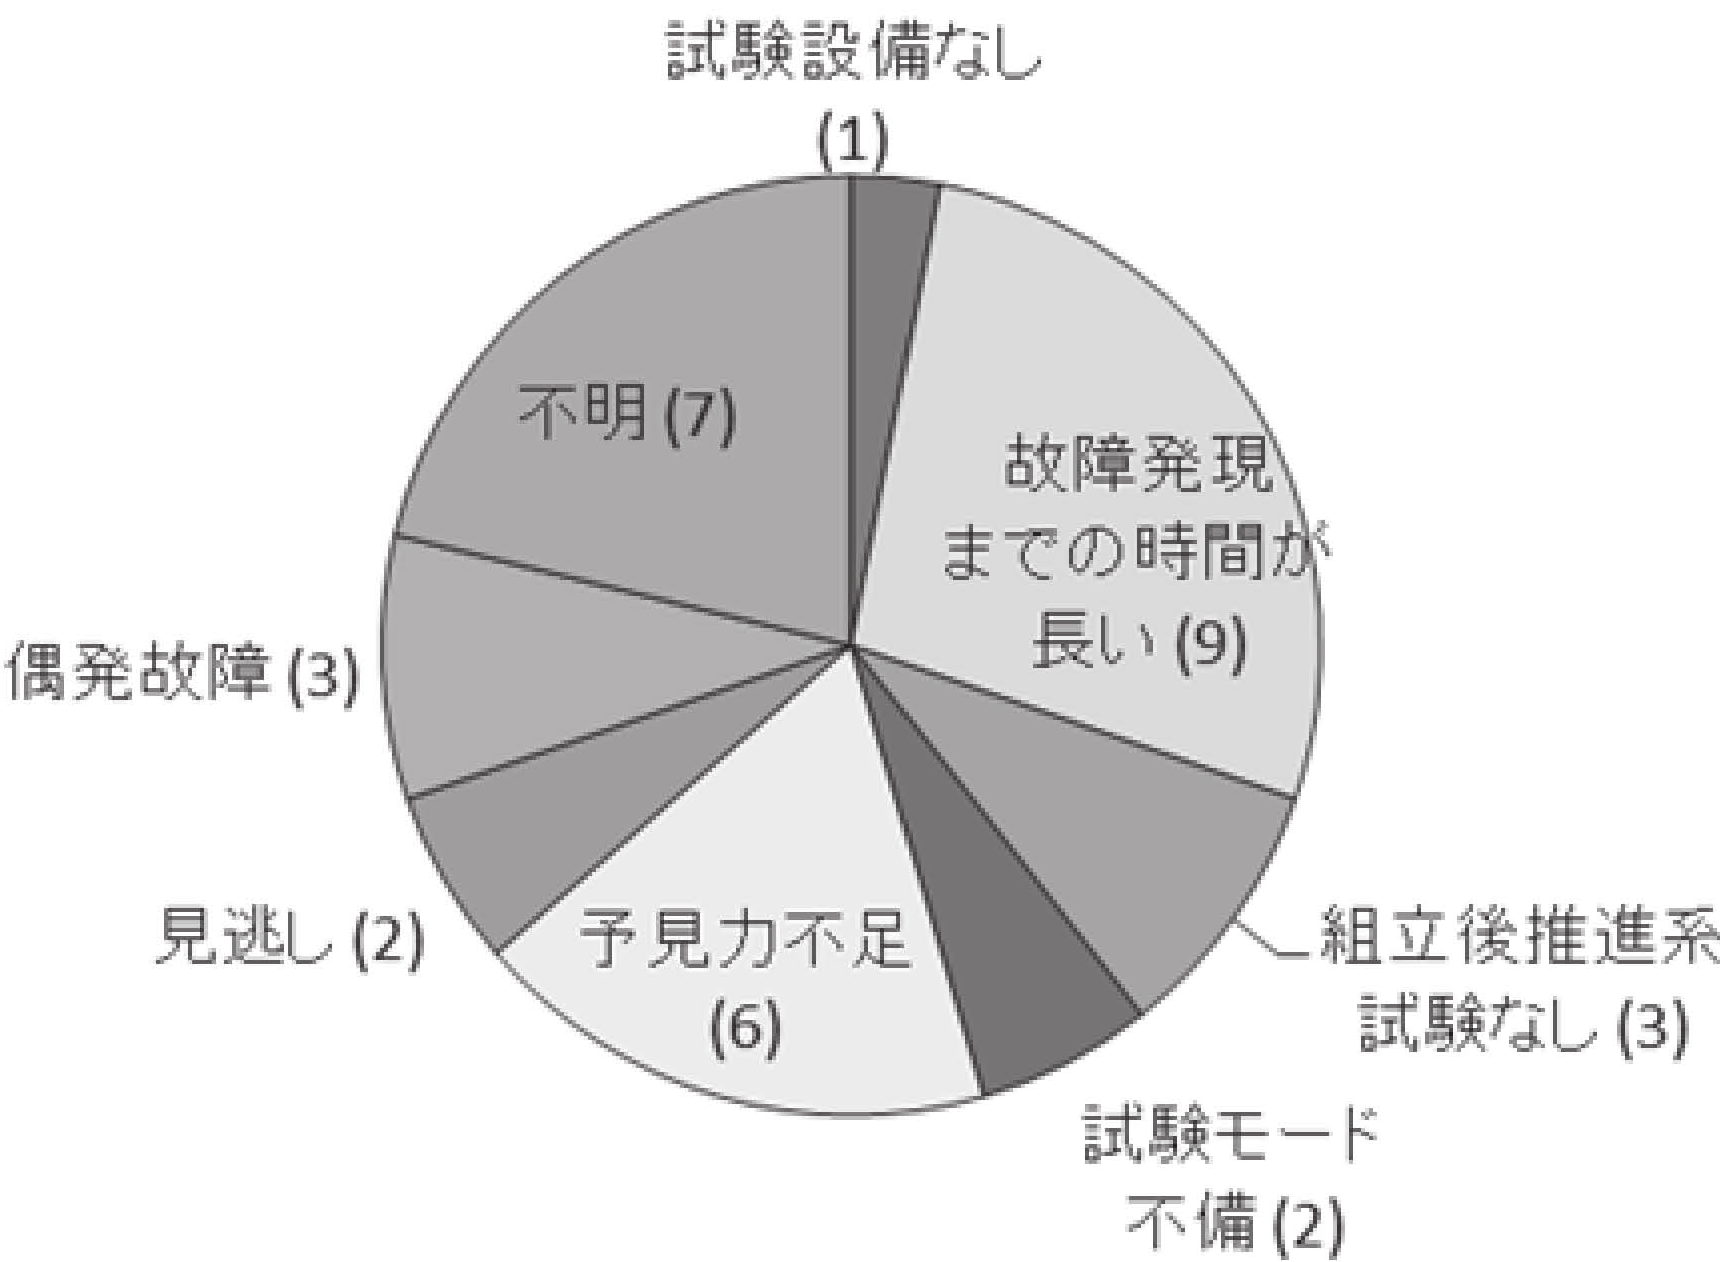
\includegraphics[height=5.5cm]{figure/not_found_error_seeds.png}
            \caption{軌道上故障の要因を地上で発見できなかった原因類型の分布\cite{SAITO2011}}
            \label{fig:error cause}
         \end{minipage}
      \end{tabular}  
\end{figure}


%ここを不具合分析の難しさに変える.
%なぜこの研究室で不具合の分析が十分に行えていなかったのかをFTA使って分析したものをベースに考えよう.
%ここの流れを見直す.根拠資料
\subsection{不具合分析の難しさ}
以上のように,衛星の不具合及びリスク分析を,
地上試験で十分に
行うことができていないという現状がある.\\
以下に人による不具合原因分析の大まかな流れを示す.
\begin{enumerate}
   \item 不具合が起きた際の衛星の状態を保存する. %これ試験の話と軌道上での話が混じってる
   \item テレメトリから考えられる故障原因の候補を洗い出す.
   \item それらの故障の中でテレメトリから分かる情報を元に候補を棄却していく.
   \item 更に切り分けが必要な場合はコマンドを送って,それに影響を受けるテレメトリによって判断する.
   \item 判断できない場合は,コンポーネントを取り出し直接確認を行う.
\end{enumerate}
%軌道上での不具合分析手法とほぼ同じである,それを活用して本手法が軌道上での不具合診断にも使えることを示す
分析が不十分になっている原因の一つとして,2の故障原因の候補
の洗い出しを網羅的に行うことの難しさがある.
組み上げ状態の衛星から得られる情報はテレメトリのみである.
この際,衛星の内部状態を理解し,テレメトリから現在の衛星の状態
を想像することができなければ,十分に不具合の原因の候補を考えることはできない.
本研究室の過去プロジェクト(PRISM)を対象にした研究では,
事前に想定していた故障モードの粒度は,
%ここの記述も微妙なので変更する
山口ら\cite{Yamaguchi2014}がモデルを用いて洗い出したものと比較して,
不十分であるという結果も出ている.
このように,人による故障モードの洗い出しは思いつきによるものなので,
考えが及んでいないことが多い.\\
また,分析が不十分になっている原因の一つとして,
3,4の故障原因の切り分け作業の難しさもある.
超小型衛星は内部状態が複雑に絡み合っており,一つの不具合に対して
非常に多くの故障候補が洗い出されることが想像できる.
そのため,多くの故障候補の中から切り分けを行い,最終的な故障を
特定するという作業は多くの知識と労力を必要とする作業である.
%切り分け作業の難しさもだが,先行研究の事例を示し,故障候補の洗い出しに関しては
%広く検討されていることを述べて,自分はこちら側をやるという方向で示せばいいのでは?

%この時,未熟な運用者が原因特定のために誤ったコマンドを送信してしまうと,
%衛星が死ぬ可能性も考えられる.このため,不具合分析を行う際には
%そのコマンドが”安全”なのかという点が非常に重要となる.

%それはそうだが,下の流れを作るためには用途に応じてコマンド選択の指標が変わることを説明したい

\section{本研究での目的}
以上を踏まえると,
不具合発生時に故障候補を洗い出し,その切り分けを行って
原因を特定していく過程に,高い知識と経験が必要になっている
ことが,
衛星の不具合やリスクの分析が不十分に
なっている原因の一つであると言える.

% 提案手法へのつながりが見えにくいため,違う記法の方がいいかもしれない.
そこで本研究では,経験が浅く,衛星に関する知識の乏しいエンジニアであっても
不具合分析を実施できるような不具合分析支援の手法を提案する.
この手法は下記の3つの要素で構成されている.
%ここも少し変わるはず,そもそもモデル化できてないし
\begin{itemize}
   \item 衛星内部のサブシステムや要素間の信号・電気・物理的相互作用のモデル化
   \item コマンド及びテレメトリによって情報が流れる経路のモデル化
   \item 不具合原因の特定を行うために必要なコマンド及びテレメトリの探索 %ここの言い回し
\end{itemize}
   
モデル化に関しては,今回は専

まずは,簡易的な衛星のモデルに対してテストケースを考え,
手法の有効性を検証し,有効であることが十分に示すことができれば,
本研究室における衛星開発で部分的に実践し有効性を
検証することを考えている.\\

\section{先行研究調査}
上述のように,不具合原因の洗い出し
が網羅的にできていないこと,仮説の検証過程が専門家等の知識依存になっていること
が不具合分析が不十分になっている原因の一つであった.%一つでないが
これらの課題に対して,古くから故障診断システムの研究が盛んに行われており,
特にモデルベースで行う手法に関して

モデルを元に不具合診断を行うシステムの研究は古くから行われており,\cite{}
正常時のコンポーネント間のつながりモデルに基づく不具合分析
手法としてGDEが広く知られている.

以下に比較結果を示す.
\begin{table}[H]
   \centering
   \caption{不具合分析手法の比較}
      \begin{tabular}{cccccc} \hline%もう少し示し方を考える.
         手法&故障網羅性&手法の目的&モデル複雑度%専門家の知識が必要という点で?
         \\ \hline
         GDE&×&故障仮説生成&低\\
         GDE+\cite{Struss1989}&△&故障仮説生成&中\\
         網状故障解析\cite{Yamaguchi2014}&△&異常モード洗い出し&高\\
         故障オントロジー\cite{Kitamura1999}&〇&故障仮説生成&高\\
         本手法&△&故障箇所切り分け&中\\ \hline
      \end{tabular}
\end{table}
%モデル複雑度が比較の指標になるのか?

%ここのところまだ実装できて無くね?
%かつ今のでできるのはON・OFF状態のアップデートだけな気がする.
故障原因の切り分けをモデルのみを用いて行うことは(論文参照する),
非現実的であり,実機の状態をフィードバックしながら対話的に
切り分けを行っていくシステムのほうが現実的である.
%何言うてるか分からん

詳細なモデルを用いて,不具合原因である機器の故障の原因などを探索可能にしたものなど
あるが,網羅的な故障仮説の洗い出しを行うことがメインであり,
実際の検証段階を組み込んだものは少ない.

また,故障診断のコンテキストによってどこまで掘り下げるべきか使い分けるべきである
\cite{Ontology1998}ことを書く.
今回の手法で扱える範囲はどこまでで,試験時に役立てることができるのか,運用時
だとどうなのかを示す.
%でもこれ書くとこはモデルと手法のアルゴリズムを示してからのほうがいいか

故障診断の全ての過程を対象の制約モデルを用いて行うことは,
対象とするモデルの粒度に非常に高い忠実度が求められるため,複雑に物理現象が絡み合う
衛星では難しい.
むしろ,人間を対話的にサポートすることによってシステムに求められるモデル化のコスト
を下げつつ,不具合分析(故障診断)の過程を体系化し,経験の少ないエンジニアの支援が
できると考えられる.


本手法では,衛星へのアクションとしてコマンドを用いながら,故障仮説の洗い出しと
検証を同時に行うことによって,用意すべきモデルに求められる粒度のレベルを下げている.
%こんな感じかな....

自分の手法の新規性を示す.

%以下で何を書くかをまとめる
%まずは手法の説明
%モデルの説明
%コマンドを評価するための指標に関して
%探索のアルゴリズムの具体的説明????
%実装結果(できればわかりやすい形で示したい)
%探索結果に関する考察
%

%検証という言葉が正しくない.検証は立てた仮説の正しさを調べること
\section{提案手法}
以下のFigure \ref{fig:fault_diagnosis}に提案手法の不具合分析を行うフローを示す.
図中において本研究の対象は,黄色に示しているところであり,
不具合発生時のコマンド送信情報とテレメトリ情報
が与えられてから,それらが通る経路の探索を行い,その経路内に
存在する故障箇所を検証するために必要な確認事項の洗い出しを行うことである.

%故障診断の方がいいかもしれない
\subsection{不具合分析アルゴリズム}
%この図も修正する.番号が下の箇条書きとかぶってややこしいから修正する.
%検証結果のフィードバックもできるようにする予定.
%ただし,OK NGという簡単なフィードバック.パラメータ的な状態量は組み込めていない

\begin{figure}[H]
   \centering
      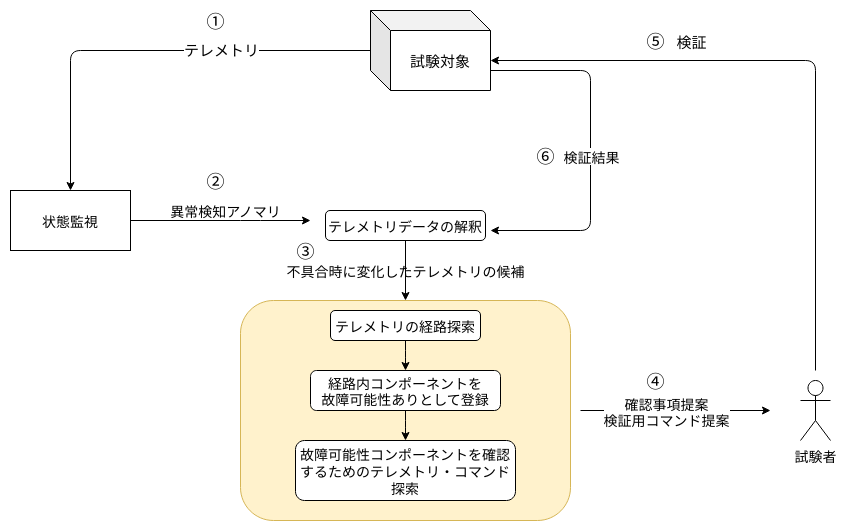
\includegraphics[height=8.0cm]{figure/fault_diagnosis_flow.png}
      \caption{不具合分析の流れ}
      \label{fig:fault_diagnosis}
\end{figure}


%フローチャートで示せるならそのほうがわかりやすいかもしれない
本手法の不具合分析の流れは以下である.
%\renewcommand{\labelenumi}{\roman{enumi}}
\begin{enumerate}
   \item 不具合検知のきっかけとなったテレメトリの候補を与える.
%   どこが異常値なのかを認識させる. 
   %不具合を起こしたトリガーが何なのかは分からないが,コマンドによってもたらされたかの区別だけ必要?
   \item そのテレメトリに影響を与えるコマンドを送信してから,
   地上局がテレメトリを受信するまでの一連の経路を取得する.
   \item 得られた経路内にあるコンポーネントを「故障候補」として登録する.(故障仮説の生成)
   %その経路に対してコマンドパスとして入力があれば,入力の元となっているコンポーネントも故障候補に追加する.
   \item 他のテレメトリを確認することによって,棄却できる「故障候補」を棄却する.
   \item コマンドを送って得られるテレメトリ情報によって,
   故障候補を棄却し,故障箇所の切り分けができるコマンドの探索を行う.
   %以下を繰り返すみたいな形にしたいけど
   \begin{enumerate}
      \item 
   \end{enumerate}
   \item 以上で得られたコマンドに関して,人が切り分けを行う際の判断の指標と共に
   提示する.
   \item システムが提示した指標を元に人が打つコマンドを選択し,仮説の検証を行う.
   \item コマンドによって返ってきた,テレメトリを確認し正常かどうかのフィードバックを行う.
\end{enumerate}


このようなアルゴリズムで不具合分析を行うためには,
以下のようなモデルが必要となることがわかった.
\begin{itemize}
   \item 各コンポーネント間の接続関係
   \item コマンド・テレメトリがコンポーネント間を伝わる経路
   \item コマンドに影響を受けるテレメトリの関係
\end{itemize}



%ここにモデルの説明
%モデル化に関しては今回研究のスコープから外す.モデルありきで行うことにした
%jsonで定義した.Component_stateとCommand_typeのモデルの話も必要になる.
%これらのモデルに基づいて,実装上ではどのようなオブジェクトが生成され
%どのように関係しているのかを図示できたほうがいい
\subsection{事前定義モデル}
次に,以上で述べたアルゴリズムで不具合分析を行うために必要なモデル
に関して,具体的なテストケースをベースにして
説明を行う.%言い回し

%これも既にモデル.先にどんなモデルが必要になるのかをまとめておいたほうがいいのか?
\subsubsection{対象とするテストケース}
今回,以下のFigure \ref{fig:simple_sat}の
ような簡易衛星モデルを考え,モデル化の手法について
述べる.\\
また,矢印の色が情報の方向性を表しており,
赤がコマンドによる情報の伝達,
青がテレメトリによる情報の伝達である.
また,矢印の種類が情報として伝わる物
を表しており,それぞれ以下のようになっている.
\begin{itemize}
   \item Signal:電気信号
   \item Power:電源
   \item Heat:熱
\end{itemize}
\begin{figure}[H]
   \centering
      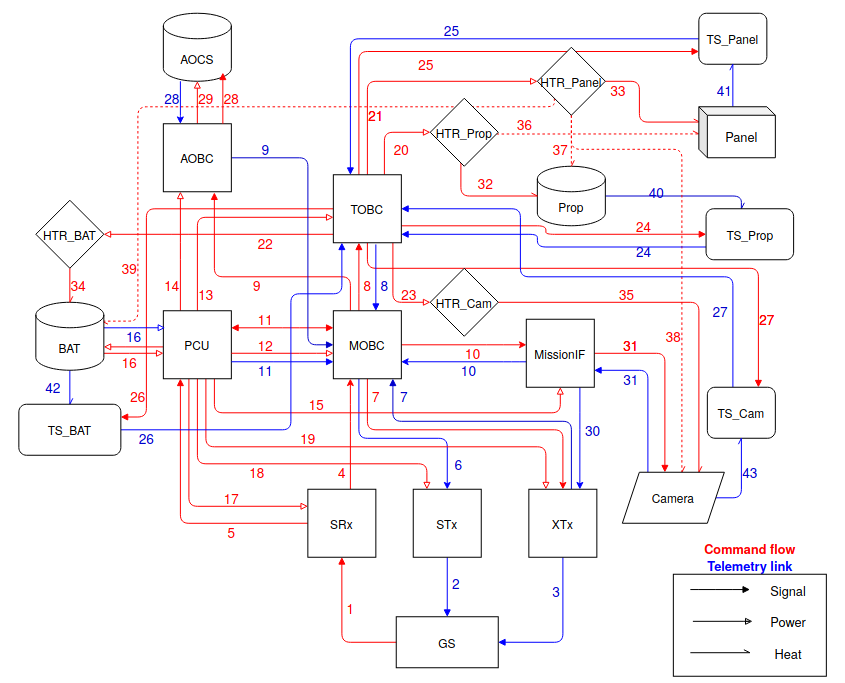
\includegraphics[height=12.0cm]{figure/satellite_diagram.PNG}
      \caption{簡易衛星モデル}
      \label{fig:simple_sat}
\end{figure}

\subsubsection{各コンポーネント間の接続関係モデル}
來村ら\cite{Kitamura01}は拡張デバイスオントロジーとして,
機器を構成する装置間のつながりを表現するために「ポート」と「導管」%ここの説明を考える
という概念を定義している.このオントロジーを用いて,山口ら\cite{Yamaguchi2014}
は人工衛星デバイスオントロジーを構築している.
%論文ではもう少し詳細に説明する.
これらを参考にし,以下のTable \ref{tab:link_definition}のように
接続関係を「リンク」として定義した.\\%違いを説明する必要があると思う
リンクが持つ情報としては,リンク名,接続コンポーネント,ID,伝達物
となっており,IDが各リンク固有の識別子としてリンクを参照する際に
使用される.また,実際にコンポーネント間を接続している実態(配線やコネクタなど)を表現している
のではなく,接続関係を概念的に表現したものにすぎない.
%そのメリットは何なん?
%ほんまはちゃんとポートと導管を作ったほうが良かったんかもしれん

\newpage
%キャプションとくっついているか確認
%図新しいのに変える
\begin{table}[H]
   \centering
   \caption{リンク定義} 
   \label{tab:link_definition}
\end{table} 
\vspace{-2zh}
\begin{figure}[H]
   \centering
      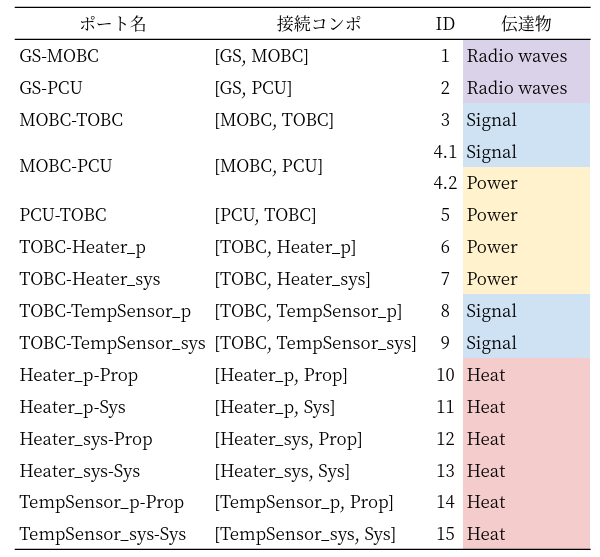
\includegraphics[height=10cm]{figure/port_definition.png}
\end{figure}
次に,コンポーネントの定義を行う.以下のTable \ref{tab:compo_link}では,
衛星システム全体として使用されている
コンポーネントのリストを作成し,各コンポーネントの属性として
コマンドリンクとテレメトリリンクを,上で定義したリンクのID
を用いて定義している.
ここで,コマンドリンクというのはコマンドによる情報の伝達で使用されるリンクであり,
テレメトリリンクというのはテレメトリによる情報の伝達で使用されるリンクである.
この時,コンポーネントが属性として持つリンクはそのコンポーネントが出力元となる場合としている.

%キャプションとくっついているか確認
%図新しいのに変える
%\newpage
\begin{table}[H]
   \centering
   \caption{コンポーネント定義} 
   \label{tab:compo_link}
\end{table}
\vspace{-2zh}
\begin{figure}[H]
   \centering
      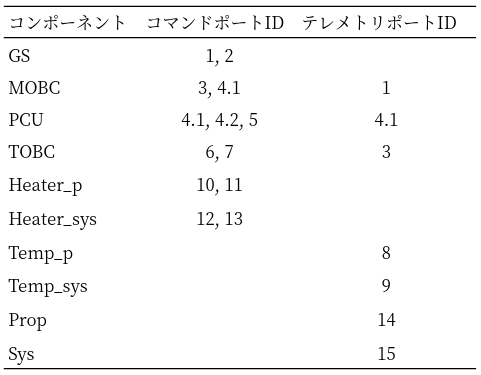
\includegraphics[height=7cm]{figure/compo_port.png}
\end{figure}

以上の情報によって,衛星内部でコンポーネント全体がどのように接続しているか
を定義することが可能になる.

また,テレメトリに含める状態量として,以下の ような各コンポーネントの状態を定義する.
%Component_stateを記述する.これスクショの方が色ついててわかりやすいな
\renewcommand{\lstlistingname}{Code}
\begin{lstlisting}[caption=コンポーネント初期状態例,label=compo_sate]
   {...
   "AOBC":{"Active":true,
		"PowerConsumption":{"value":2,"unit":"W"},
		"Heat":"+",
		"Function":{}},
	"MIF":{"Active":true,
		"PowerConsumption":{"value":1,"unit":"W"},
		"Heat":"+",
		"Function":{"Get_Data":{"Active":false,"target":"CAM","PowerConsumption":0}}},
	"PCU":{"Active":true,
		"PowerConsumption":{"value":1,"unit":"W"},
		"Heat":"+",
      "Function":{}},
      ...}
\end{lstlisting}
%どっちにするか選択
\begin{figure}[H]
   \centering
      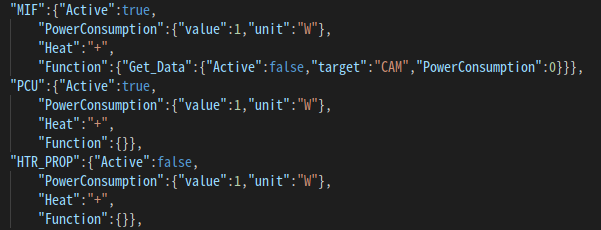
\includegraphics[height=5.0cm]{figure/Component_state.png}
      \caption{コンポーネント初期状態例}
      \label{fig:Compo_state}
\end{figure}

本研究では簡単のため状態量として扱うものは,各コンポーネントの電源状態,
それに伴う電力消費,姿勢変化及び,熱の発生としている.
また,電源ON/OFF状態以外にも機能を持つコンポーネントは
Functionという概念を追加し,
%将来的にはパラメータを含む状態量も扱えるように拡張していく予定である.

\subsubsection{コマンド・テレメトリの情報がコンポーネント間を伝わる経路のモデル}
次に,コマンド及びテレメトリがコンポーネント間を伝わる経路を探索するために
必要なコマンド及びテレメトリの定義に関して述べる.
まず,今回の衛星モデルにおいて使用できるテレメトリ及びコマンド
を以下のTable \ref{tab:telemetry},\ref{tab:command}に示す.

%経路だけじゃなくて,遷移するトリガーも加えたことを記述
%これ書くのクソだるいので図にして貼る.それかなんかCSVからできるやつ使う
\begin{table}[H]
   \centering
   \caption{使用テレメトリ}
   \label{tab:telemetry}
      \begin{tabular}{cllcccc} \hline
         ID&テレメトリ&経路\\ \hline
         1&MOBCカウンター&MOBC$\rightarrow$GS\\
         2&MOBC電流値&PCU$\rightarrow$MOBC$\rightarrow$GS\\
         3&TOBCカウンター&TOBC$\rightarrow$MOBC$\rightarrow$GS\\
         4&TOBC電流値&PCU$\rightarrow$MOBC$\rightarrow$GS\\
         5&推進系温度&Prop$\rightarrow$TempSensor\_p$\rightarrow$TOBC$\rightarrow$MOBC$\rightarrow$GS\\
         6&システム温度&Sys$\rightarrow$TempSensor\_sys$\rightarrow$TOBC$\rightarrow$MOBC$\rightarrow$GS\\
         7&推進系ヒータ電流値&TOBC$\rightarrow$MOBC$\rightarrow$GS\\
         8&システムヒータ電流値&TOBC$\rightarrow$MOBC$\rightarrow$GS\\
         9&MOBCコマンドカウンター&MOBC$\rightarrow$GS\\
         10&TOBCコマンドカウンター&TOBC$\rightarrow$MOBC$\rightarrow$GS\\ \hline
      \end{tabular}
\end{table}

%コマンドのTypeを定義したことに関しても
%ここも修正
\begin{table}[H]
   \centering
   \caption{使用コマンド}
   \label{tab:command}
      \begin{tabular}{clllccc} \hline
         ID&コマンド&経路&影響テレメトリID\\ \hline
         1&MOBC電源ON&GS$\rightarrow$PCU$\rightarrow$MOBC&1,2,9\\
         2&MOBCコマンドカウンターアップ&GS$\rightarrow$MOBC&9\\
         3&TOBCコマンドカウンターアップ&GS$\rightarrow$MOBC$\rightarrow$TOBC&10\\
         \multirow{2}{*}{4}&\multirow{2}{*}{推進系ヒータON}&GS$\rightarrow$MOBC$\rightarrow$PCU$\rightarrow$TOBC&\multirow{2}{*}{5,6,7}\\
         &&$\rightarrow$Heater\_p$\rightarrow$(Prop,Sys)&\\
         \multirow{2}{*}{5}&\multirow{2}{*}{システムヒータON}&GS$\rightarrow$MOBC$\rightarrow$PCU$\rightarrow$TOBC&\multirow{2}{*}{5,6,8}\\
         &&$\rightarrow$Heater\_sys$\rightarrow$(Prop,Sys)&\\
         6&TOBC電源ON&GS$\rightarrow$PCU$\rightarrow$TOBC&3,4,10\\ \hline
      \end{tabular}
\end{table}

今回,Table \ref{tab:telemetry}に示すテレメトリの経路及び,Table \ref{tab:command}
に示す経路と影響テレメトリIDに関しては事前に定義したものを使用した.
%より曖昧なつながりを考え波及効果を考えていくためにはどうするべきかについても言っておきたい

%コマンドのタイプ(これも名前が不適切かもしれないが,)に関しても言及する.
%故障箇所でなく,不具合原因という言葉にする?
また,コマンドに対するテレメトリの応答を確認して不具合原因を絞り込んでいくためには
コマンドがテレメトリ情報に変化をもたらす必要がある.

\cite{}

実際の衛星ではコンポーネント数やコマンド・テレメトリの数
が膨大であるためモデルが複雑化し,人によるモデル生成では
ヒューマンエラーや,作業量を考えると非現実的である.
そのため,将来的にはこれらを必要最低限の情報から生成する手法に関しても
検討していく.

\subsection{コマンド評価指標}
次に,上記のアルゴリズムによって切り分けを行う際,
人間がコマンドを選択するための指標に関して説明する.
本研究の当初の目的は地上試験においての不具合分析支援であったが,本手法は
コマンドとテレメトリの粒度で得られる情報を用いて不具合分析を行っているので,
軌道上の運用時にも活用できると考えられる.
そのため,地上試験時と運用時の両方に関してコマンドを選択する上で必要な指標を
提案し,
使用状況に合わせて評価指標を切り替えることのできるフレームワークであることを示す.
%指標に関する説明

\subsubsection{負の効果}
%衛星開発及び運用の経験がある方々へのヒアリングの結果,
不具合分析を行う際,衛星の安全を確保しながら確実に切り分けを行えることが
重要である.
%そうとは限らない
そのためには,不具合発生時の状態をなるべく変えないように
しながら徐々に切り分けを行っていくことが必要である.
そこで,コマンドによって発生する
衛星内部状態の変化の大きさを定量的に示し,そのコマンド
の「負の効果」を表現することにする.\\
まず,状態量の変化

各コンポーネントに定義された状態を変化させる
%これを示す前にどんな衛星を元にしていて,どのような仮定をしているのかを示さないと意味がわからない.
各コマンドを打つことによる状態量の変化として,以下のものが有用であると考えた.
\begin{itemize}
   \item 変化する状態量の数
   \item コマンドを打つ前のバッテリ残量と,コマンドを打つことによって発生する消費電力
   \item 姿勢変化を起こすか否か
\end{itemize}

\subsubsection{正の効果}

また,運用時には
可視時間が限られていて,その可視パス中に不具合原因を究明しなければいけないような時間制約
がある場合がある.その際には,少ないコマンド数で効率的に原因特定が行えることが望ましい.
そのため,以下のようにコマンドの「正の効果」を定義した.\\
%どれだけのリンク(故障候補)を確認できるかという点
コマンドの効果として重要なのは,コマンドを送ることによって
確認できる故障候補がいくつ存在するかという点である.これは絞り込むことのできる
能力を表していると言える.

%リンクの定義.あとここで言っている正常はつながりが切れていないかという点であることを説明する.
各コマンドによって情報が伝達し,テレメトリとして地上局に返ってくる経路によって,
確認する対象のリンクまでに通る経路が異なる.%ココらへんの図が必要そう
その各経路に存在するコンポーネントをつなぐリンクが正常である確率を
$P(l = \text{normal})$,異常である確率を$P(l = \text{abnormal})$ %確率Pも斜体じゃないほうがええかも
として与える.
あるリンク$l_i$を確認するためには,リンク$l_i$が接続されているコンポーネントまでの経路
が正常であることが必要である.このことから,「リンク$l_i$を確認することができる確率」
がそれぞれの経路によって定まる.このことを以下のFigure \ref{fig:route}に示す例を用いて示す.\\
\begin{figure}[H]
   \centering
      \begin{tabular}{c}
         \begin{minipage}{0.50\hsize}
         \centering
         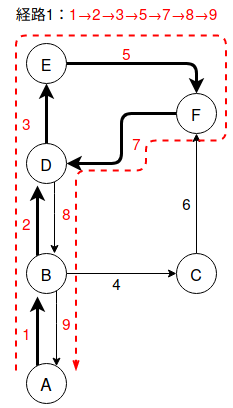
\includegraphics[height=8cm]{figure/route1.png}
          %  \caption{}
            \label{fig:route1}
         \end{minipage}
         \begin{minipage}{0.50\hsize}
         \centering
         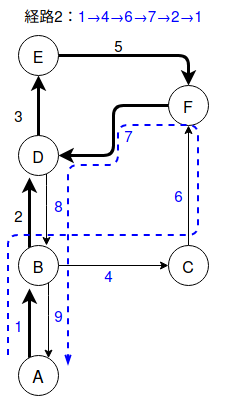
\includegraphics[height=8cm]{figure/route2.png}
         %\caption{}
            \label{fig:route2}
         \end{minipage}
      \end{tabular} 
      \caption{故障候補とそれを確認するための情報伝達経路の例}
      \label{fig:route}
\end{figure}
以下では簡単のため,$P(l_i = \text{normal}) = P(l_i = \text{abnormal}) = 0.5$であるとし,
太矢印になっている箇所が故障候補である.故障候補以外は正常であるとし,
$P(l_i = \text{normal}) =1$である.
この時,リンク7を確認するためにはノードAからノードFまでの経路(1,2,3,5)
が正常である必要がある.%正常の定義を明確に
ここで,経路を表す記号をR,経路内にある故障候補リンクの集合を$\mathbb{F}$とすると,
経路1を通る情報でリンク$7$を確認することができる確率は
\begin{eqnarray}
   P(l_{7} | \text{R}_1) &=& \prod_{i\in\mathbb{F}_1,i\neq 7} P(l_{i} = \text{normal})\\
     &=& \left( \frac{1}{2}\right)^4
\end{eqnarray}
であることが分かる.ここで,R$_1$は経路1,また
\begin{eqnarray}
   \mathbb{F}_1  &=& \{ 1,2,3,5\} 
\end{eqnarray}
である.\\
同様に経路2に関してもリンク$7$を確認することができる確率は
\begin{eqnarray}
   P(l_{7} | \text{R}_2)  &=& \prod_{i\in\mathbb{F}_2,i\neq 7} P(l_{i} = \text{normal})\\
   &=& \frac{1}{2}
\end{eqnarray}
となる.

これを元に考えると,コマンドが通る経路によって,
故障候補コンポーネントに接続しているリンクが正常であるかを確認できる
数の期待値$E(\text{R})$は以下のように求まる.
\begin{eqnarray}
   E(\text{R})&=& \sum_{i\in \mathbb{F}}P(l_i|\text{R})
   = \sum_{i\in \mathbb{F}}\prod_{j\in \mathbb{F}, j\neq i} P(l_j=\text{normal}) \label{eq:E(R)}
\end{eqnarray}
これが,あるコマンドとそれによって影響を受けるテレメトリとで形成される
経路を伝達する情報によって確認することのできるリンク数の平均を示している.
つまり,コマンドが不具合原因を絞り込むことのできる能力を表していると言える.
よって,その経路の「正の効果」を示す指標の一つとして式(\ref{eq:E(R)})を確認可能リンク数
として定義する.\\
ここで,Figure \ref{fig:route}の経路1(R$_1$とする)と経路2(R$_2$とする)に関して計算してみると
\begin{eqnarray}
   E(\text{R}_1)  &=& P(l_{1} | \text{R}_1) + P(l_{2} | \text{R}_1) +P(l_{3} | \text{R}_1)
   +P(l_{5} | \text{R}_1) + P(l_{7} | \text{R}_1) \\
   &=& 1 + \frac{1}{2} + \left( \frac{1}{2}\right)^4 + \left( \frac{1}{2}\right)^4
    + \left( \frac{1}{2}\right)^4 \\
    &=& 1.6875 \\
   E(\text{R}_2)  &=& P(l_{1} | \text{R}_2) + P(l_{7} | \text{R}_2) \\
   &=& 1 + \frac{1}{2} \\
   &=& 1.5
\end{eqnarray}
結果からわかるように,通る経路に存在する故障候補の数
が必ずしも確認できるリンクの数に対応しているわけではない.
故障候補のリンクを通ることで不確定性が蓄積されるため,より末端側の
リンクを確認できる確率は小さくなる.そのため,経路1のような多くの故障候補を通る経路は,
その経路内に含まれる故障候補の数(4)と,確認できるリンクの数の期待値(1.6875)の差が大きくなる.\\
一方で,経路2のように通る経路に含まれるリンクの多くが正常であると分かっている場合は,
経路内に含まれる故障候補の数(2)と,確認できるリンクの数の期待値(1.5)が近くなっており,
対象をより確実に確認できる経路であると言える.

このことを踏まえて,あるコマンドとテレメトリのペアによって形成される経路(R)を通る情報によって
故障候補の確認を行う際,経路内に含まれる故障候補の数($N_F$とする)と
確認できるリンクの数の期待値($E$(R))の割合が,その経路が対象とする故障候補
の内どれだけ確認することができるかを示している.
上で述べたように,切り分けを行っていくためには確実性が重要である.%ちゃんと上で述べる
そのため,その経路の「正の効果」を示す指標の一つとして確実性($C$(R)とする)を以下のように定義する.
\begin{eqnarray}
   C(\text{R})  &=& \frac{E(\text{R})}{N_F}
\end{eqnarray}
%ここらへん実装まで終わらして,ちゃんと有効であることを示せないと伝わらなさそう.
%有効でなければやり直しやが..

以上では,コマンドとそれによって影響を受けるテレメトリとのペアによって形成される経路に対して
「正の効果」を定義していたが,各コマンドが影響を与えるテレメトリは複数存在することが多くある.
人間が選択する際にはコマンドに対して指標が必要である.\\
あるコマンドに関連する経路が複数ある場合,それらに関する「確認可能リンク数」及び「確実性」
の単純和を取るだけでは対象としているリンクに被りが生じるため,コマンドの効果を表している
とは言えない.
そこで,各経路で被りが生じているリンクに関しては,
そのリンクを通る経路の中で距離が最短な経路が確認を行うものとし上の指標を再定義を行う.
あるコマンド(COMとする)が影響を与える各テレメトリと成す経路の集合を
$\mathbb{R} = \{ \text{R}_1, \cdots ,\text{R}_{N} \}$(ただし$N$はコマンドCOMによって形成される経路の数,
また$\mathbb{R}$は経路長さの昇順でソートされている)とする.
また,$\mathbb{R}$に含まれる故障候補の集合を,各経路(R)$_i$に含まれる故障候補
の集合$\mathbb{F}_i$の直和を取り%少し間違っているから修正
%なんかいい方法思いつかんから保留
\begin{eqnarray}
    \mathbf{F} &=& \sum_{i=1}^N \mathbb{F}_i
%    \bigcup_{i=1}^N \left( \bigcup_{i=1}^N \mathbb{F}_i - \bigcap_{i=1}^N\right) 
\end{eqnarray}
とし,$\mathbf{F}$に含まれるリンクの数を$\mathbf{N_F}$とする.
この時,COMの「確認可能リンク数」及び「確実性」は以下のようになる.
\begin{eqnarray}
   E(\text{COM})  &=&\sum_{i\in \mathbf{F}} \prod_{j\in \mathbf{F}, j\neq i} P(l_i=\text{normal})  \\
   C(\text{COM})  &=& \frac{E(\text{COM})}{\mathbf{N_F}}
\end{eqnarray}
これらをコマンドの「正の効果」を表す指標として定義し,人間にの判断を支援するシステム
を構築する.
%ここに情報量を組み込むといいかも?めんどくさい

%ここ洗練させる
\subsubsection{評価指標の使い分け}
次に,地上試験と軌道上での運用でどのように上述した指標を使い分けるのかについて
説明する.

今回,故障候補の洗い出しは研究対象ではないため,簡単に不具合検知のきっかけとなった
テレメトリが通る経路としており,それ以外の経路は正常であるという仮定をする.

\begin{comment}
   
%エントロピー使うなら平均は取らない.
まず,コマンドを打つことによってどれだけの情報が得られるかという点から,
そのコマンドを打つことによる情報量を考えた.

その指標として,コマンドの能力を情報量(エントロピー)の定義から考えた.
無理にエントロピーを使うのは間違っている気がする.情報量という考え方が妥当ではないか?
確率分布になっていないことを考えると.

コマンド$j$による切り分けの効果の指標を以下に定義する.\\
コマンド$j$が確認できるリンクの集合を$\mathbb{L}_j$とする.
この時,集合に含まれるリンクは$l_i\in \mathbb{L}_j$とする.
また,
「$\mathbb{L}_j$を確認する」という事象を$\Omega$とすると,
各リンク$l_i$を確認するという事象$E_i \in \Omega$として,

ここで,各リンクの状態を確認する方法として,本手法ではコマンドによるアクセスのみを考えているので
「リンク$l_i$を確認する」という事象と,「リンク$l_i$を確認できるコマンドを選択する」
という事象の確率は等価である.%各コマンドを選ぶ確率は等しいという仮定が入っているような気がする.
よって,「リンク$l_i$を確認する」という事象の確率は式(\ref{eq:Pi})
で与えられる.この時,事象($E_i$)が起こった時に受け取る(選択)情報量$I_i$は式(\ref{eq:I_i})
で定義される.

\begin{eqnarray}
   P(E_i) &=& \frac{\text{Number of command which can verify Link }i}{\text{All command number}} \label{eq:Pi}\\
   I(E_i) &=& -\log{P_{i}} \label{eq:I_i} \\
\end{eqnarray}
確率$P(E_i)$は確率分布であるという説明が必要

よって事象$\Omega$による平均情報量は
\begin{eqnarray}
   H(P) &=& -\sum_{E_i \in \Omega} P(E_i)\log{P(E_i)} 
\end{eqnarray}
となる.定性的な意味としては,コマンドを打つことによってどれだけの情報
が得られる可能性があるかを示している.

コマンドが絞り込むことのできる能力という点はどうする?

以上の指標を踏まえた上でどのように提示し人間の判断を支援するのかを考える.
\end{comment}
%地上試験と運用時の両方で使い分けることのできるフレームワークであることを示す.
地上試験時は,不具合原因の特定を時間を掛けて十分に行いたいので,
衛星の安全を担保しながら確実な箇所から切り分けを行うことが重要である.
%確実な箇所とは?
不具合分析を行う過程で,内部状態が大きく変化してしまうと切り分けたい故障箇所
がわからなくなってしまう可能性があるため,
確実に切り分けを行っていくためには,コマンドによって変化する状態量
が少ないことが望ましい.
よって,地上試験では「波及効果の大きさ」が小さなコマンドを用いて
切り分けを行っていくことが望ましい.\\
一方で,運用中は可視時間中に不具合原因の特定を行わなければならないなどの
時間制約の厳しい条件下での分析が必要になることもある.
そのような時には,リスクを大きく取りつつ効果の大きなコマンドを選択する必要がある.

また,試験では考慮しない電力による制約も,コマンドを選択する際の
一つの指標であると言える.

このように,コマンドによって不具合特定を行っていく際には,評価指標を
使い分けることができるようなシステムである必要がある.


%ここは実際の実装の中でのアルゴリズム?別に必要ないかな?
%実践した結果を分かりやすく表示させるように変更して,その結果を例に説明するのがいいかもしれない
\subsection{各故障を切り分けていくための確認事項の探索}
次に,故障候補の中から切り分けを行っていくためのアルゴリズムに関して
検討状況を述べる.
不具合が発生している状態で予期せぬ二次故障を起こさないために,
探索順序としては,
衛星の状態を変えずに確認できるものを優先的に探索
することが望ましい.\\ 
%ここ表現がわかりにくい
そこで,不具合発生時に取得しているテレメトリデータの中から
故障原因特定に役に立つテレメトリ情報が存在するなら,
そのテレメトリを確認事項として提案する.
%ここの流れは上のアルゴリズムのところで述べたのでは?
また,衛星の状態を変化させること無く
故障原因特定のために得られる情報がなくなれば,
次ステップとしてコマンドを打って得られる
情報から切り分けを行っていくことになる.
このとき,残ったコマンドで故障候補の状態を確認できるものを探索し,
上で示した指標の計算を行う.提示するコマンド候補としては,
使用するコンテキストに適した評価指標に基づいて
上位 のコマンドを指標の値とともに提示する.

%ここは実践例
\subsection{問題設定}
最後に,不具合分析の具体的な流れをみるために,以下のような故障を考え,
不具合分析を行っていく.\\
まず,MOBCとTOBCからテレメトリは全て降ろされているものと仮定する.
また,故障は「推進系ヒータの接着不良」であるとする.
その時,テレメトリを通して確認できるのは
\begin{itemize}
   \item 「推進系ヒータON」コマンドを送ったのに,「推進系温度」テレメトリが変化しない.
\end{itemize}
という事象である.
よって不具合検知は,この事象によって行われる.

\subsubsection{不具合分析の例}
この不具合において,「推進系ヒータON」コマンドを送信して推進系ヒータに熱が伝わるまでの経路
と,推進系温度計が温度を読み取り「推進系温度」テレメトリとして地上局に伝わるまでの
経路の中に故障箇所があると考えることができる.
この経路を以下のFigure \ref{fig:simple_sat_fault}に太矢印で示している.
%これにリンクID入れたら見やすいかも
\begin{figure}[H]
   \centering
      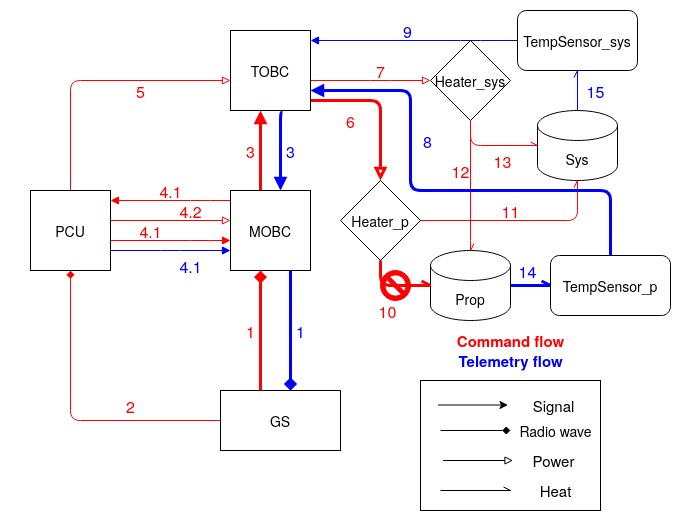
\includegraphics[height=9.0cm]{figure/simple_sat_fault.png}
      \caption{故障箇所と不具合検知に関連するコマンドとテレメトリの経路}
      \label{fig:simple_sat_fault}
\end{figure}
また,この経路内にあるコンポーネントに電源が入っているかどうかを確認するためには,
そのコンポーネントに電源を供給するための経路が正常に作動しているかどうかを確認する
必要がある.そこで
\begin{itemize}
   \item PCU$\rightarrow$MOBC(リンクID:4.2),PCU$\rightarrow$TOBC(リンクID:5)
\end{itemize}
も検証を行う対象として考える.
以上より,検証すべき経路は下記のようになる.
\begin{itemize}
   \item コンポーネント:GS,MOBC,TOBC,Heater\_p,Prop,TempSensor\_p
   \item コマンドリンク:GS-MOBC(1),MOBC-TOBC(3),MOBC-PCU(4.2),
   PCU-TOBC(5),\\TOBC-Heater\_p(6),Heater\_p-Prop(10)
   \item テレメトリリンク:GS-MOBC(1),MOBC-TOBC(3),TOBC-TempSensor\_p(8),
   TempSensor\_p-Prop(14)
\end{itemize}
以下,提案手法によるアルゴリズムによって不具合分析を行っていく.\\
%この章長くて読みにくい
まず,問題設定よりMOBC及びTOBCのテレメトリは全てダウンリンクされている状態に
あるので,
\begin{itemize}
   \item テレメトリリンク:TOBC$\rightarrow$MOBC(3),MOBC$\rightarrow$GS(1)
   \item コマンドリンク:PCU$\rightarrow$MOBC(4.2),PCU$\rightarrow$TOBC(5)
\end{itemize}
は問題ないことが確認できるため,故障可能性はなくなる.
問題設定ではあるが,実際に「MOBC及びTOBCのテレメトリが全てダウンリンクされている」
ことを確認するためには,「MOBCカウンター」
「TOBCカウンター」を確認することが必要である.\\
また不具合発生時,推進系ヒータが正常に作動しており,
システム温度計からテレメトリを下ろす経路に問題がなければ,
「システム温度」が上昇しているはずである.
よって,テレメトリの確認によって検証できる経路として,
コマンドリンク「TOBC-Heater\_p(6)」がある.
以上より,不具合発生時から状態変化させずに確認すべき事項として以下
が挙げられる.

\begin{table}[H]
   \centering
   \caption{コマンドなしでの確認事項} 
   \label{tab:check_list1}
\end{table}
\vspace{-2zh}
\begin{figure}[H]
   \centering
      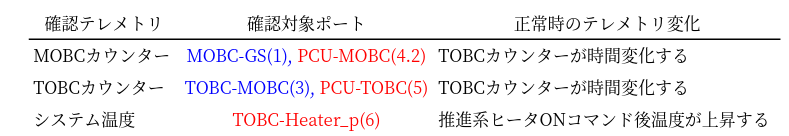
\includegraphics[height=2.5cm]{figure/check_list_tel.png}
\end{figure}
衛星の状態を変化させること無く,テレメトリを確認するだけで
検証できる箇所はこれ以上存在しないので,次にコマンドによる検証を行う.

まず,コマンドパスとしてGSに近い箇所から順に確認を行う必要がある.
MOBCへのコマンドが通っているかを確認するためには,「MOBCコマンドカウンターアップ」
コマンドを送って,「MOBCコマンドカウンター」が変化していることを確認できれば良い.
同様に考えると,以下の様に確認事項を洗い出すことができる.
\begin{table}[H]
   \centering
   \caption{コマンド送信による確認事項} 
   \label{tab:check_list2}
\end{table}
\vspace{-2zh}
\begin{figure}[H]
   \centering
      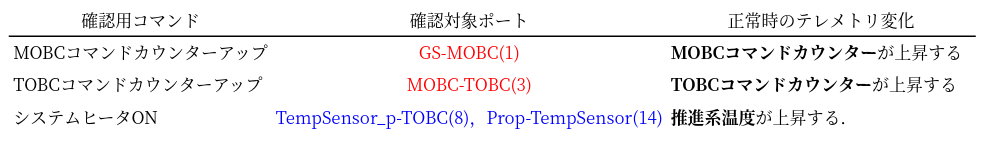
\includegraphics[height=2.6cm]{figure/check_list.png}
\end{figure}
以上の項目を確認した際,今回想定した故障モード(推進系ヒータの接着不良)
では期待されるテレメトリデータの変化が起こるので,
Table \ref{tab:check_list2}の確認対象パスの中にある故障可能性箇所は
棄却され,
故障可能性リンクとして残るのは
\begin{itemize}
   \item コマンドリンク:Heater\_p-Prop(10)
\end{itemize}
となる.

%上のコマンドを送っても大丈夫なのかという議論はどうするのか?もしシステム温度が高いのに,その方法でたしかめてもいいものなのか?

この経路上で考えうる故障モードと照らし合わせると,
この切り分けによって残る故障モードは
\begin{itemize}
   \item 推進系ヒータの故障
   \item 推進系ヒータの接着不良
\end{itemize}
となる.
この時,
「システム温度」の上昇によって「推進系ヒータの故障」の可能性は
棄却できるため,最終的に「推進系ヒータの接着不良」
が残り,
実際の故障を棄却すること無く,絞り込みができていると言える.\\

%今後の方針とかいるんかよ.どのように卒論にまとめていきたいか
%以上の不具合分析の流れを参考にし,探索のアルゴリズムを考えたい.
\section{今後の方針}

また,熱や運動のような支配方程式が微分方程式で定義されており,
単純なつながりだけでは表現できないような現象に関しては,
この手法では簡易的に表現することしかできていない.
そのため,この手法を物理現象が複雑に絡んだ不具合分析に適用することは難しい.
将来的には,これらの支配方程式を解く
シミュレータを組み込むことによって複雑な物理現象も扱えるように
手法の改良が必要である.

%評価軸を示して,この手法の有効性をどのように示す予定かをのべる.

\bibliographystyle{junsrt} %何がええかは考える plain, acm, alpha とか
\bibliography{Ref} 
\end{document}